% Template for APA submission with R Markdown

% Stuff changed from PLOS Template
\documentclass[a4paper,man,apacite,floatsintext]{apa6}
\usepackage{apacite}

% amsmath package, useful for mathematical formulas
\usepackage{amsmath}
% amssymb package, useful for mathematical symbols
\usepackage{amssymb}

% hyperref package, useful for hyperlinks
\usepackage{hyperref}

% graphicx package, useful for including eps and pdf graphics
% include graphics with the command \includegraphics
\usepackage{graphicx}

% Sweave(-like)
\usepackage{fancyvrb}
\DefineVerbatimEnvironment{Sinput}{Verbatim}{fontshape=sl}
\DefineVerbatimEnvironment{Soutput}{Verbatim}{}
\DefineVerbatimEnvironment{Scode}{Verbatim}{fontshape=sl}
\newenvironment{Schunk}{}{}
\DefineVerbatimEnvironment{Code}{Verbatim}{}
\DefineVerbatimEnvironment{CodeInput}{Verbatim}{fontshape=sl}
\DefineVerbatimEnvironment{CodeOutput}{Verbatim}{}
\newenvironment{CodeChunk}{}{}

% cite package, to clean up citations in the main text. Do not remove.
\usepackage{cite}

\usepackage{color}

% Use doublespacing - comment out for single spacing
%\usepackage{setspace}
%\doublespacing


% Text layout
\topmargin 0.0cm
\oddsidemargin 0.5cm
\evensidemargin 0.5cm
\textwidth 16cm
\textheight 21cm

% Bold the 'Figure #' in the caption and separate it with a period
% Captions will be left justified
\usepackage[labelfont=bf,labelsep=period,justification=raggedright]{caption}


% Remove brackets from numbering in List of References
\makeatletter
\renewcommand{\@biblabel}[1]{\quad#1.}
\makeatother


% Leave date blank
\date{}

%\pagestyle{myheadings}
%% ** EDIT HERE **


%% ** EDIT HERE **
%% PLEASE INCLUDE ALL MACROS BELOW

%% END MACROS SECTION


% ALL OF THE TITLE PAGE INFORMATION IS SPECIFIED IN THE YAML
\title{\textbf{Children's reasoning about honest versus polite speakers}}
\shorttitle{Children's reasoning about politeness}

\author{Erica J. Yoon, Michael C. Frank}

\affiliation{Department of Psychology, Stanford University}

\authornote{The Author Note, containing contact information, acknowledgements, etc}
\abstract{Abstract text.}
\keywords{If provided, keywords will be displayed on a line beneath the abstract.}

\begin{document}
\maketitle

\section{Introduction}\label{introduction}

\section{Experiment 1A}\label{experiment-1a}

\subsection{Method}\label{method}

\subsubsection{Participants}\label{participants}

Parents and their 5-6- and 7-8-year-old children visiting Children's
Discovery Museum in San Jose, CA, were invited to participate in a short
study. \ldots{}FIXME\ldots{} These exclusion criteria led to a final
sample of 26 5-6-year-olds and 19 7-8-year-olds.

Adult participants were recruited through Amazon Mechanical Turk.
\ldots{}FIXME\ldots{} These exclusion criteria led to a final sample of
50 adult participants that were included in the analysis.

\subsection{Results and Discussion}\label{results-and-discussion}

\begin{CodeChunk}

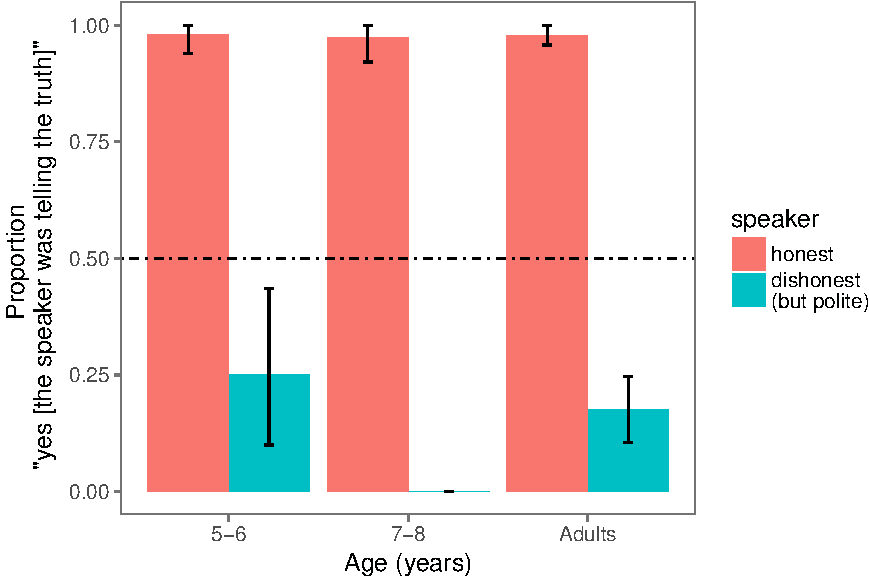
\includegraphics{figs/unnamed-chunk-1-1} \end{CodeChunk}

\begin{table}[h]
\centering
\begin{tabular}{lrrr}
 Predictor & Estimate & Std. Error & $z$ value \\ 
  \hline
Intercept & 4.35 & 1.28 & 3.40 \\ 
  8-year-olds & -0.21 & 1.83 & -0.11 \\ 
  Adults & 0.00 & 1.48 & 0.00 \\ 
  Polite speaker & -5.95 & 1.32 & -4.50 \\ 
  8-year-olds * Polite speaker & -111.26 & 11032629.28 & -0.00 \\ 
  Adults * Polite speaker & -0.37 & 1.53 & -0.24 \\ 
   \hline
\end{tabular}
\caption{Predictor estimates with standard errors and significance information for a generalized linear mixed-effects model predicting speaker truth-telling judgments} 
\label{tab:nice_tab}
\end{table}

Across all age groups, adults and children correctly judged the honest
speaker to be telling the truth, and the polite speaker as not telling
the truth. A generalized linear mixed-effects model predicting
truth-telling judgment based on age and speaker type showed a
significant main effect of speaker type (\(\beta\) = -5.95,
\(p <.001\)). There was no main effect of age, and no interaction
between age and speaker type. Thus, even the youngest group of
participants we tested were able to correctly reason that the honest
speaker was telling the truth, whereas the polite speaker was lying.

\begin{CodeChunk}

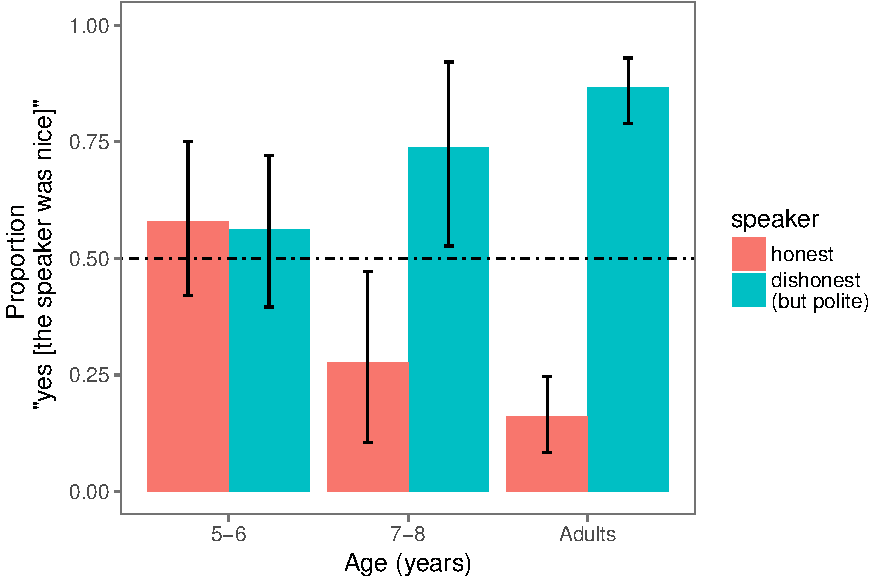
\includegraphics{figs/unnamed-chunk-2-1} \end{CodeChunk}

\begin{table}[h]
\centering
\begin{tabular}{lrrr}
 Predictor & Estimate & Std. Error & $z$ value \\ 
  \hline
Intercept & -1.21 & 0.55 & -2.19 \\ 
  6-year-olds & 1.63 & 0.72 & 2.26 \\ 
  Adults & -1.01 & 0.64 & -1.57 \\ 
  Polite speaker & 2.56 & 0.65 & 3.92 \\ 
  6-year-olds * Polite speaker & -2.59 & 0.82 & -3.16 \\ 
  Adults * Polite speaker & 2.17 & 0.78 & 2.79 \\ 
   \hline
\end{tabular}
\caption{Predictor estimates with standard errors and significance information for a generalized linear mixed-effects model predicting speaker niceness judgments} 
\label{tab:nice_tab}
\end{table}

There was a clear developmental trend in judgments of speaker niceness.
Whereas adults and 7-8-year-olds judged the polite speaker to be nice
and the honest speaker to be not nice (\(|t|\) \textgreater{} -2.77,
\(p <0.009\)), 5-6-year-olds did not judge either speaker to be nice or
not nice (\(|t|\) \textless{} 1.04, \(p >0.302\)), not differentiating
between the two speaker types. A generalized linear mixed-effects model
predicting niceness judgment based on age and speaker type revealed a
significant interaction between age and speaker type (6-
vs.~8-year-olds: \(\beta\) = -2.59, \(p =.002\); 8-year-olds vs.~adults:
\(\beta\) = 2.17, \(p =.005\)). These findings show that as children
grow older, they become more adult-like in their judgment of the polite
but dishonest speaker as ``nice''.

Then what underlie these changes in judgments as children grow older?
There are two possible interpretations: One possible explanation is
older children are more proficient at inferring other people's mental
states (Wellman \& Liu, 2003), leading them to place more weight on the
addressee's feelings in evaluating a white lie or blunt truth. Since a
white lie would make the addressee feel good, older children may have
reasoned that the polite lie-teller was being nice, whereas younger
children did not reach that level of reasoning.

Another possibility is that younger and older children use different
communicative goals; younger children may prioritize honesty, which
caused them to judge lie-tellers as not nice relatively more often,
whereas older children value politeness more.

\begin{CodeChunk}

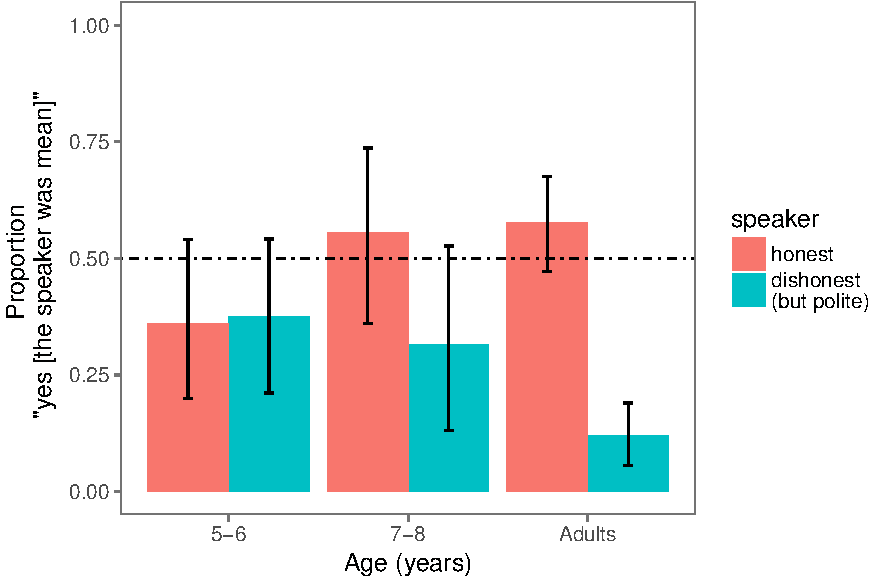
\includegraphics{figs/unnamed-chunk-3-1} \end{CodeChunk}

\begin{table}[h]
\centering
\begin{tabular}{lrrr}
 Predictor & Estimate & Std. Error & $z$ value \\ 
  \hline
Intercept & 0.21 & 0.53 & 0.40 \\ 
  6-year-olds & -1.19 & 0.73 & -1.64 \\ 
  Adults & 0.25 & 0.60 & 0.42 \\ 
  Polite speaker & -1.21 & 0.58 & -2.10 \\ 
  6-year-olds * Polite speaker & 1.57 & 0.78 & 2.02 \\ 
  Adults * Polite speaker & -2.03 & 0.71 & -2.85 \\ 
   \hline
\end{tabular}
\caption{Predictor estimates with standard errors and significance information for a generalized linear mixed-effects model predicting speaker meanness judgments} 
\label{tab:nice_tab}
\end{table}

The judgments of speaker meanness also revealed a developmental trend
that resembled that for the niceness judgment, though to a lesser
extent. Whereas adults tended to judge the honest speaker (i.e.~blunt
truth-teller) to be mean (\(t\)(141) = 1.86, \(p =0.065\)) 5-6-year-olds
tended to judge in the opposite direction (\(t\)(44) = -2.35,
\(p =0.024\)). 7-8-year-olds' judgments did not differ from chance
(\(t\)(34) = 0.5, \(p =0.619\)). On the other hand, adults and
7-8-year-olds tended to judge the polite speaker to be not mean
(7-8-year-olds: \(t\)(36) = -2.25, \(p =0.031\)), whereas 5-6-year-olds'
judgments did not differ from chance. Thus, older participants tended to
judge the blunt truth-teller to be mean and the white lie-teller to be
nice, whereas 5-6-year-olds did not, if not leaning toward the opposite
direction.

\begin{CodeChunk}

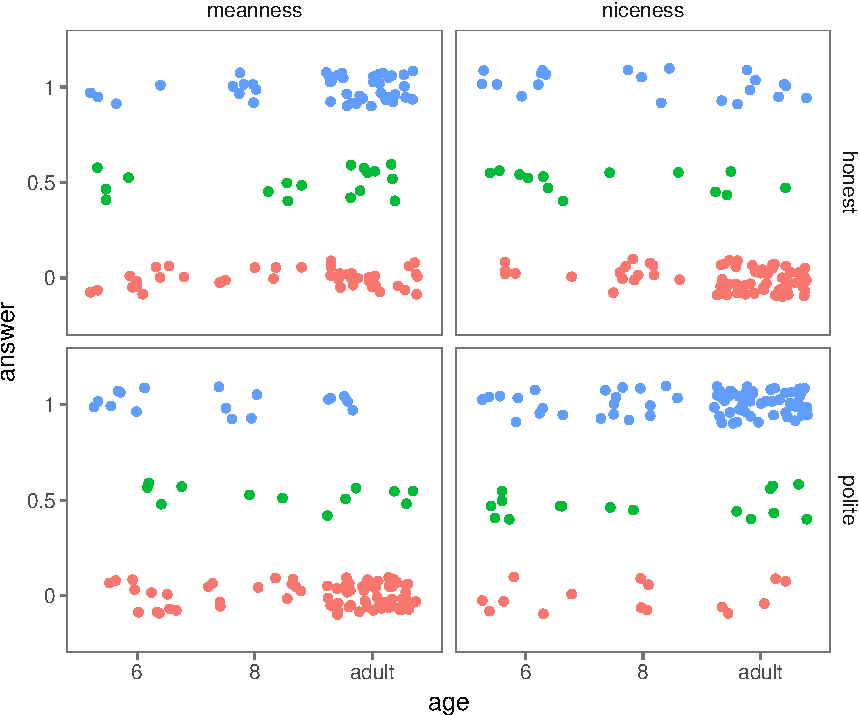
\includegraphics{figs/unnamed-chunk-4-1} \end{CodeChunk}

\section{Experiment 1B}\label{experiment-1b}

\subsection{Method}\label{method-1}

\subsection{Results and Discussion}\label{results-and-discussion-1}

\begin{CodeChunk}

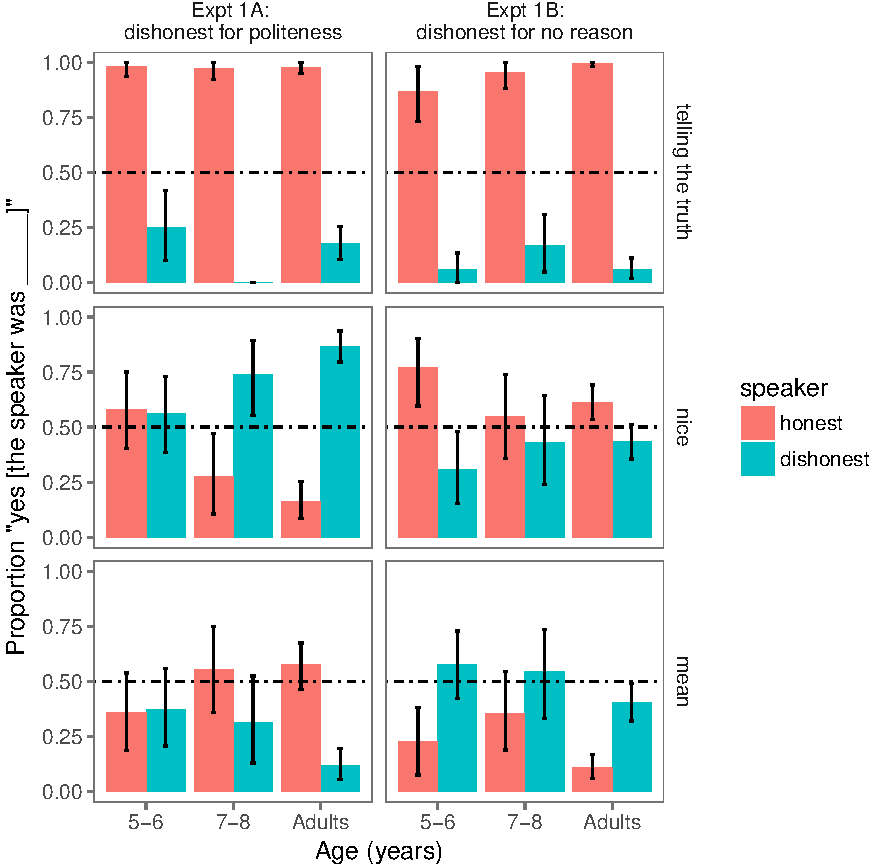
\includegraphics{figs/unnamed-chunk-6-1} \end{CodeChunk}

\begin{table}[h]
\centering
\begin{tabular}{lrrr}
 Predictor & Estimate & Std. Error & $z$ value \\ 
  \hline
Intercept & 0.21 & 0.35 & 0.60 \\ 
  6-year-olds & 1.17 & 0.51 & 2.28 \\ 
  Adults & 0.28 & 0.39 & 0.72 \\ 
  Polite speaker & -0.52 & 0.46 & -1.13 \\ 
  6-year-olds * Polite speaker & -1.78 & 0.67 & -2.65 \\ 
  Adults * Polite speaker & -0.26 & 0.52 & -0.50 \\ 
   \hline
\end{tabular}
\caption{Predictor estimates with standard errors and significance information for a generalized linear mixed-effects model predicting speaker niceness judgments for Expt 1B} 
\label{tab:1b_mean_tab}
\end{table}

\begin{table}[h]
\centering
\begin{tabular}{lrrr}
 Predictor & Estimate & Std. Error & $z$ value \\ 
  \hline
Intercept & -0.70 & 0.41 & -1.72 \\ 
  6-year-olds & -0.96 & 0.60 & -1.61 \\ 
  Adults & -1.68 & 0.51 & -3.31 \\ 
  Polite speaker & 0.93 & 0.49 & 1.89 \\ 
  6-year-olds * Polite speaker & 1.16 & 0.71 & 1.64 \\ 
  Adults * Polite speaker & 1.00 & 0.59 & 1.71 \\ 
   \hline
\end{tabular}
\caption{Predictor estimates with standard errors and significance information for a generalized linear mixed-effects model predicting speaker meanness judgments for Expt 1B} 
\label{tab:1b_mean_tab}
\end{table}

For the truth-telling judgments in Experiment 1B, children and adults
showed similar response pattern to Expt 1A: they judged the honest
speaker as truth-telling and dishonest speaker as not truth-telling. For
the niceness judgments, however, the results were the reverse of the
findings in Expt 1A: whereas adults and 7-8-year-olds overall tended to
judge neither speaker to be nice or not nice (with the exception of
adults judging the honest speaker to be nice above chance),
5-6-year-olds judged the honest speaker to be nice and dishonest speaker
to be not nice (\(|t|\) \textgreater{} -3.06, \(p <0.004\)).

\section{References}\label{references}

\bibliography{library.bib}

\end{document}
